\subsection*{Punto 03}

\textbf{Para cada k, calcule y muestre en una gráfica el indice (score) Calinski Harabasz (CH) calculado para los datos de entrenamiento. Muestra CH como una función de k, y comente al respecto. Que valor de k maximiza este criterio?}

\begin{figure}[H]
    \centering
    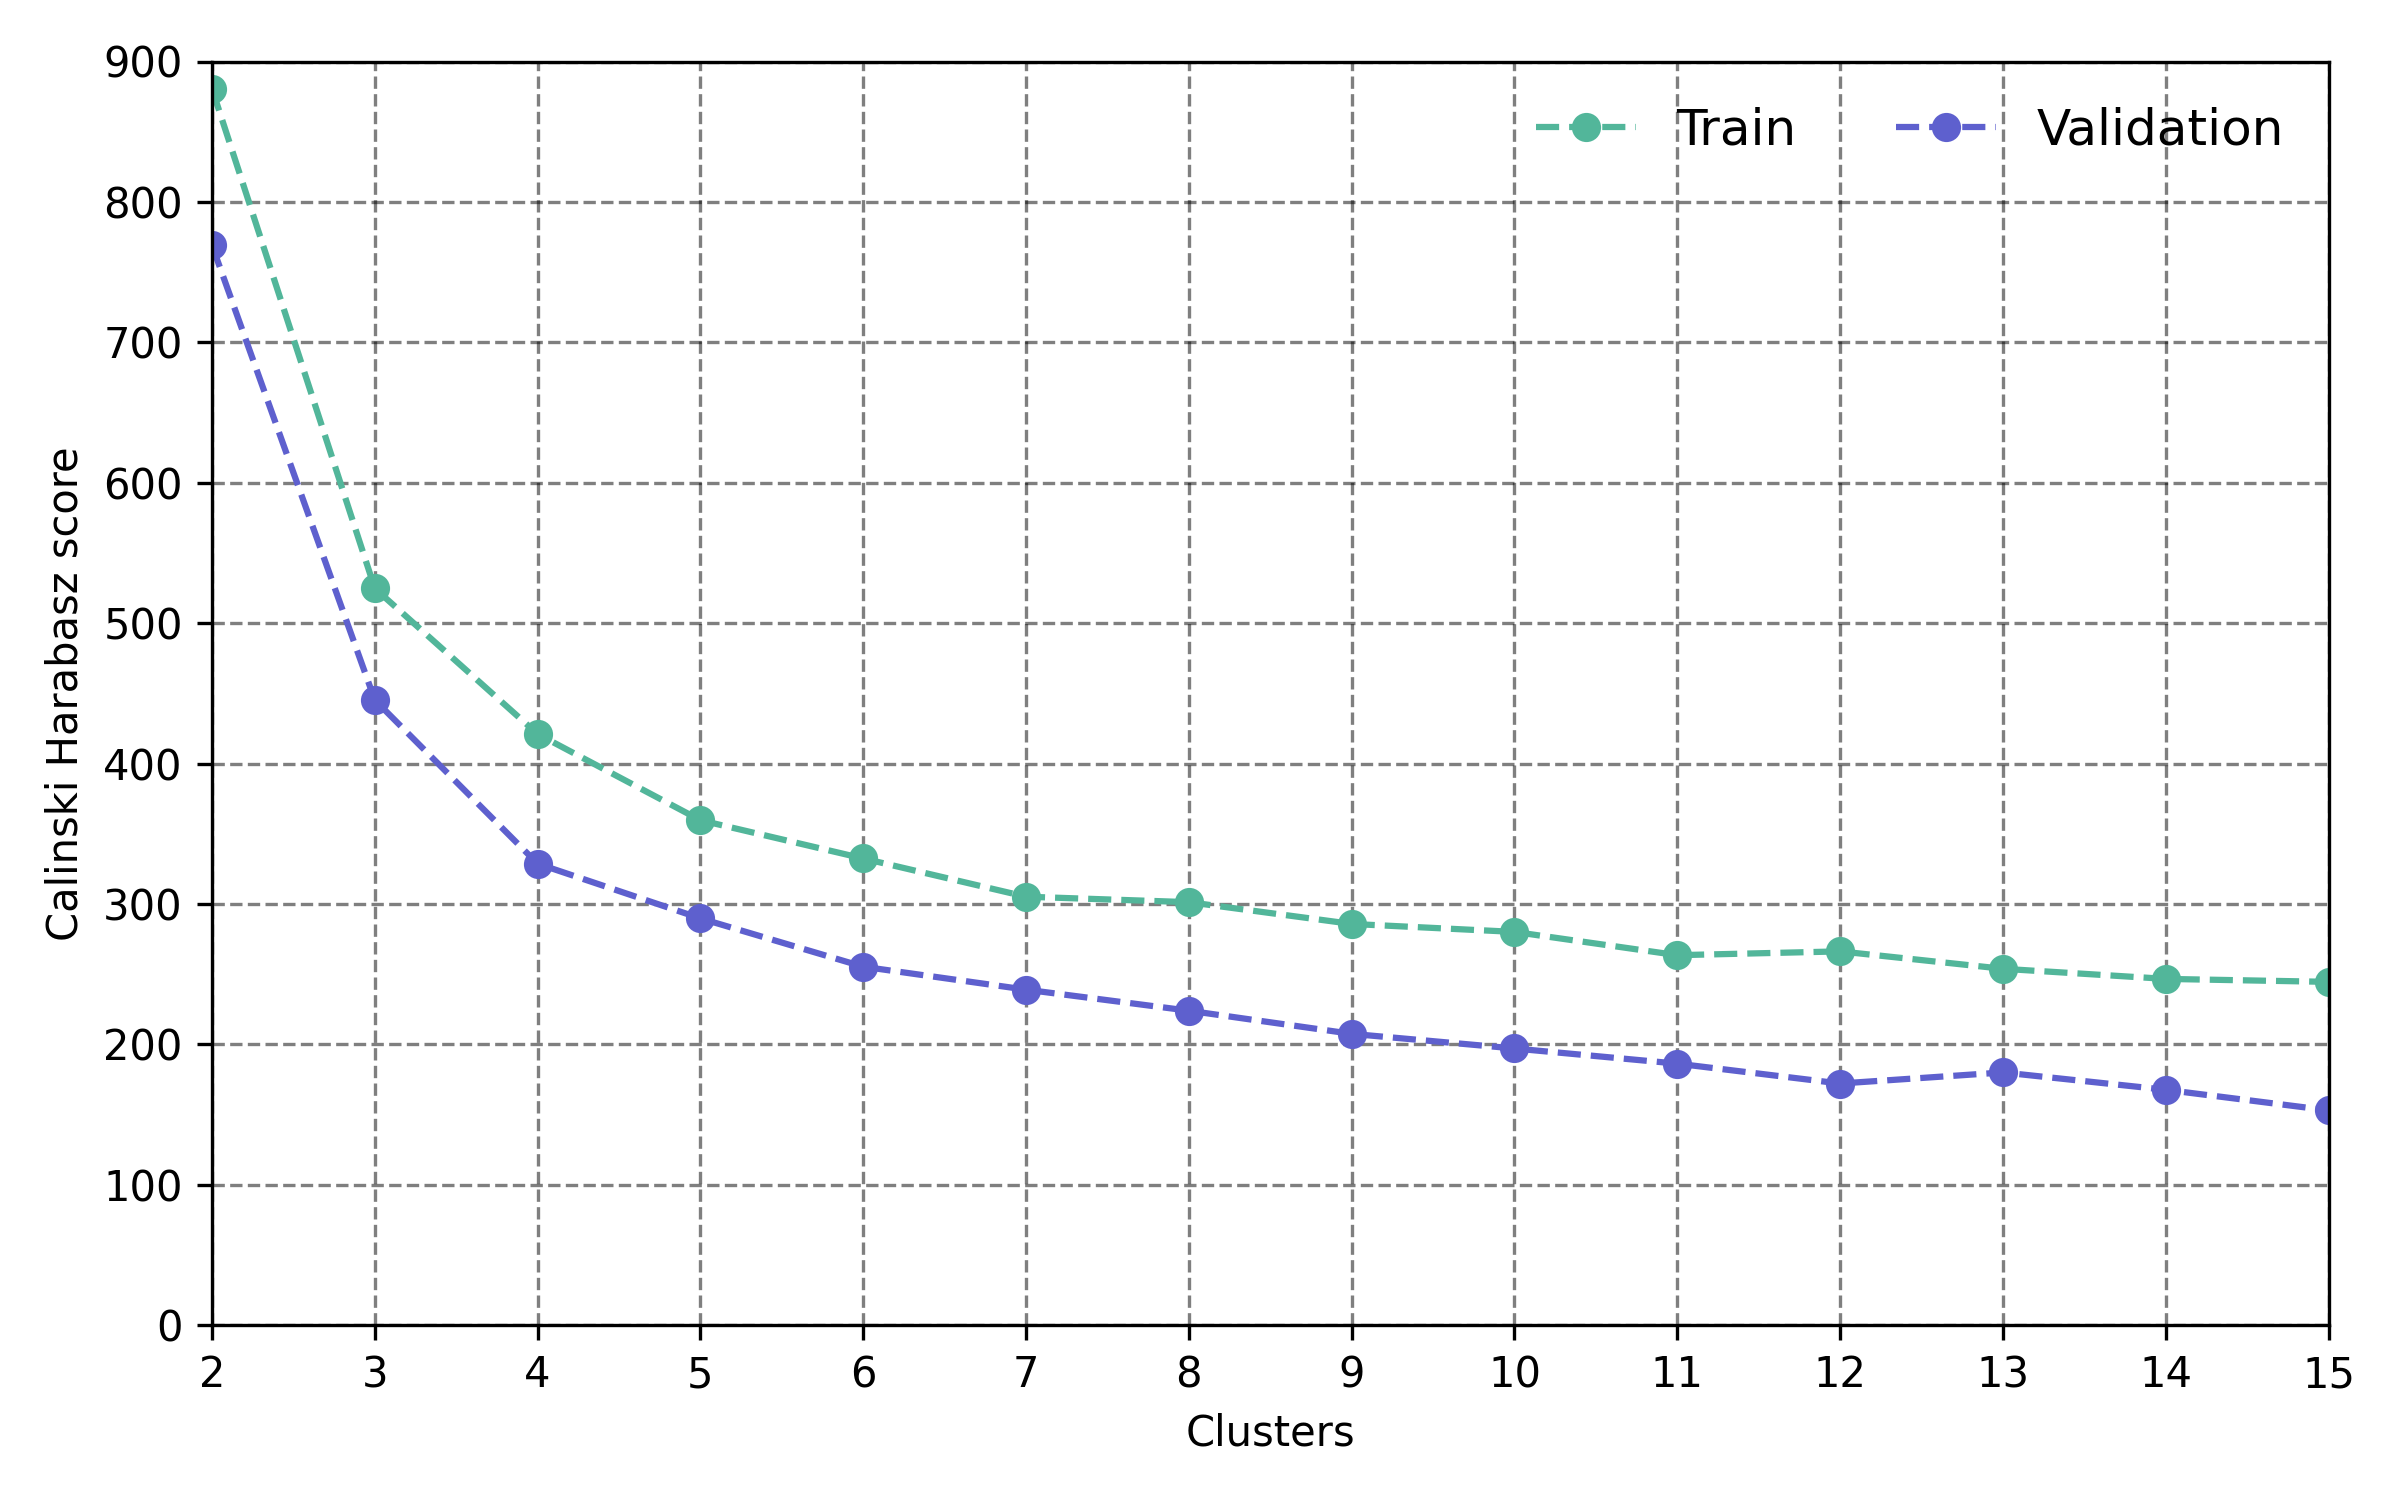
\includegraphics[width=15cm]{Graphics/Problema_03/calinski_harabasz_score.png}
    \caption{Índice de Calinski Harabasz obtenido a partir de la predicción de los datos de entrenamiento y validación.}
    \label{fig:problema_03_calinski_score}
\end{figure}